\documentclass[tikz,border=3pt]{standalone}
\usetikzlibrary{arrows.meta,positioning}

\begin{document}
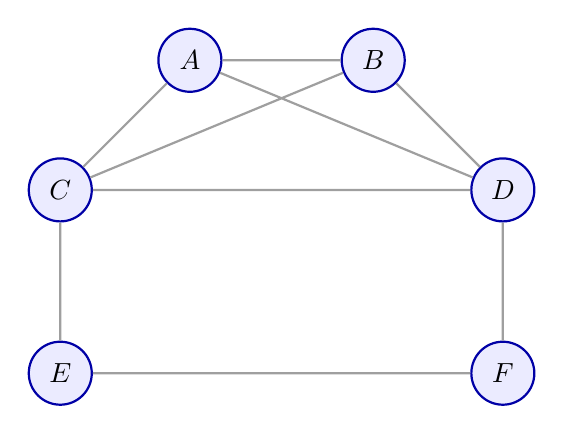
\begin{tikzpicture}[
  node distance=1.5cm,
  vertex/.style={circle, draw=blue!65!black, fill=blue!8, thick, minimum size=8mm, inner sep=1pt},
  edge/.style={draw=gray!75, thick},
]
  \node[vertex] (a) {$A$};
  \node[vertex, right=of a] (b) {$B$};
  \node[vertex, below left=of a] (c) {$C$};
  \node[vertex, below right=of b] (d) {$D$};
  \node[vertex, below=of c] (e) {$E$};
  \node[vertex, below=of d] (f) {$F$};
  \draw[edge] (a) -- (b) (a) -- (c) (a) -- (d)
    (b) -- (c) (b) -- (d) (c) -- (d)
    (c) -- (e) (d) -- (f) (e) -- (f);
\end{tikzpicture}
\end{document}
